\chapter{Introdução}

\section{Contextualização}

Na contemporaneidade são estudados diversos fatores que influenciam no crescimento e sucesso de empresas baseadas em soluções tecnológicas. Grandes empresas de prestação de serviço e venda online que tem como foco a interação de seus itens com seus clientes consideram de suma importância para seu sucesso seu sistema de recomendação.

Esse sistema tenta predizer a preferência que um dado usuário teria por um item por meio de ferramentas e técnicas de software \cite{souza:2014}. A maioria das empresas, por exemplo, utilizam de técnicas como \textit{collaborative filtering} (filtro colaborativo), que procura predizer a utilidade de itens de comércio para um cliente em particular, baseando-se na avaliação de um cliente por uma determinada amostra ou população de outros clientes, ou seja, a recomendação gerada se baseia na similaridade entre os clientes \cite{Linden:2003}.

Segundo Ricci et al. (\citeyear{Ricci:2010}) há vários motivos para fornecedores investirem nessa tecnologia, tais como:

\begin{itemize}
    \item Aumentar o número de itens vendidos;
    \item Vender itens mais diversos;
    \item Aumentar a satisfação do cliente;
    \item Aumentar a fidelidade do usuário;
    \item Melhor entendimento do que o usuário quer.
\end{itemize}

Existem diversas multinacionais que utilizam o mecanismo de recomendação em seus serviços, principalmente como forma de melhorar a interação do usuário e aumentar seu potencial financeiro. Isso vem crescendo aceleradamente de 4 a 5 anos, e há indícios que continue assim nos próximos anos \cite{Underwood:2017}.

Negócios populares e de grande porte como Netflix, Amazon, Ebay, Walmart, Costco, Spotify, Youtube e outros, são conhecidos pelos seus ótimos sistemas de recomendação. Tais empresas fazem grandes investimentos nesse tipo de tecnologia, com a finalidade de obter um retorno financeiro ainda maior \cite{Underwood:2017}.

A empresa Netflix é uma provedora internacional de séries e filmes online e se destaca entre as empresas de mídias mais bem-sucedidas financeiramente da atualidade. Graças a sua enorme quantidade de dados, foi possível criar um mecanismo de recomendação muito eficiente, no qual 75 a 80 por cento de todo o conteúdo assistido é proveniente desse mecanismo, contra os 20 a 25 por cento assistidos que são oriundos de pesquisa \cite{Kleinman:2014}. O sistema de recomendação é tão relevante para essa empresa que ela criou um campeonato, o Netflix \textit{Prize}, em que o desafio era melhorar a qualidade da recomendação, sendo que a equipe vencedora “\textit{BellKor's Pragmatic Chaos}” melhorou em pouco mais de 10\% e recebeu um prêmio no valor de 1 milhão de dólares \cite{netflixprize:2009}.

Com o crescente uso e prevalência da internet, os \textit{web services} se tornaram uma tendência. Empresas que necessitam vender seus produtos optam por utilizar plataformas virtuais, virtuais, ou como mais popularmente são conhecidos, os \textit{e-commerces}.

O mercado de varejo se deu muito bem com o comércio virtual. A Amazon, por exemplo, domina o comércio eletrônico varejista, sendo responsável por quase 50 por cento de todas as vendas online nos Estados Unidos em 2018 gerando 207 bilhões de dólares em operações de varejo pelo mundo \cite{JAKE:2019}.

O comércio de negócios para consumidores provou um aumento excelente nos últimos 15 anos, tornando o \textit{e-commerce} algo comum na vida das pessoas \cite{Jiang:2015}. Segundo a Forrester Research, vendas de varejo \textit{online} da América Latina atingirão 129 bilhões de dólares até 2023 \cite{Forrester:2019}.

Essa tendência também atingiu o mercado imobiliário. Segundo o \textit{The American National Association of Realtors} (NAR), pesquisa sobre tecnologias online, conduzida em 2011, indicou que quando se trata de busca por um lar, 88\% de compradores de imóveis escolhem a internet como fonte de informações \cite{Yuan:2013}.

O rápido crescimento de empresas de vendas online atrai atenção de investidores e gera um ambiente propício a competição. Para garantir o sucesso de um \textit{e-commerce} é de extrema importância a busca de novos recursos para garantir novos compradores e a retenção de antigos \cite{Jiang:2015}. 

Intitulado como maior \textit{e-commerce} de imóveis do Japão, o Summo.jp presa sempre em melhorias na experiência do usuário. Dentre todos os elementos de seu sistema que podem melhorar a experiência de seus usuários, o Summo.jp considera seu sistema de recomendação como o mais importante e por isso tentam sempre melhorá-lo. Seus usuários normalmente pesquisam e navegam em diversas páginas antes de encontrar um imóvel que os satisfaçam, podendo-se resultar em um processo cansativo e acabando em desistências. Recentemente, o Summo.jp passou por uma evolução e construiu um novo
sistema de recomendação baseado nos dados gerados nas pesquisas e navegações do usuário, melhorando consideravelmente sua métrica de qualidade \cite{Summo:2017}.

Buscando adotar uma abordagem semelhante, essa proposta procurará oferecer serviços diversos para imobiliárias, no qual um ambiente de \textit{e-commerce} personalizado possibilitará que os clientes dessas imobiliárias possam ter acesso e visualizar informações relativas aos diversos imóveis disponíveis para venda, agendar visitas, requisitar mais informações e verificar propriedades sobre aqueles imóveis que cada cliente tenha mais interesse.

A Liva é uma \textit{startup} que oferece serviços no ramo imobiliário e colaborará neste projeto TCC. Seus criadores são donos de grandes imobiliárias e estão trabalhando nesse ramo a mais de 36 anos. Essa situação corresponde a um dos fatores motivacionais para a elaboração desse projeto.

Um dos principais serviços fornecidos pela Liva.vc corresponde ao \textit{e-commerce} de vendas de imóveis para clientes de diversas imobiliárias, sendo mostrado na Figura \ref{fig:pagina_principal_liva} uma das janelas de acesso a este ambiente virtual.

\begin{figure}[H]
    \centering
    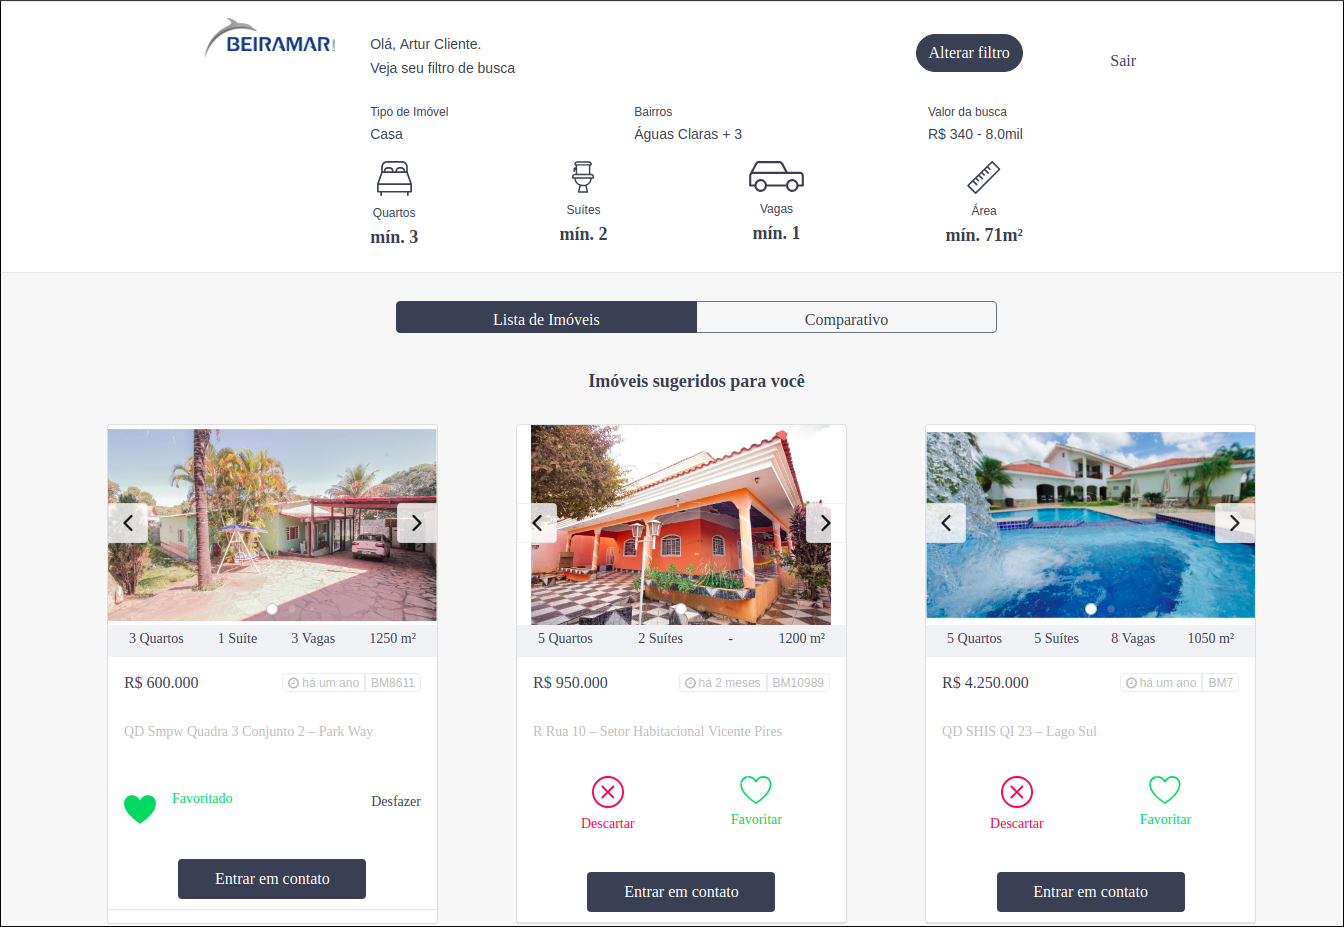
\includegraphics[scale=0.3]{figuras/introducao/pagina_principal_liva.png}
    \caption[Página principal da plataforma Liva.vc]{Página principal da plataforma Liva.vc. Fonte: \cite{Liva:2019}.}
    \label{fig:pagina_principal_liva}
\end{figure}


Esse tipo de serviço oferece um sistema de recomendação de propriedades baseado nas preferências de cada cliente. Essas preferências são primeiramente geradas a partir de um \textit{lead}. Em termos gerais, essa expressão \textit{leads} corresponderia aos clientes em potencial, ou seja, pessoas que demonstraram interesse por algum tipo de produto ou serviço, assim tornando-o um cliente interessado em algo oferecido por um negócio \cite{Agenciakaizen:2019}.

Com os \textit{leads} gerados das plataformas diariamente em grandes quantidades, diversos usuários são postos a se tornarem clientes em potencial no Liva.vc. Com dados advindos de interações de usuários com a plataforma, é possível extrair diversas informações úteis que possibilitam ainda mais refinar a preferência de cada usuário.

O processo de Mineração de Dados (\textit{Data Mining}), que é formado por diversas ferramentas e técnicas, possibilita a exploração de dados e sua extração, que ajudam a evidenciar padrões e dessa forma auxiliam na descoberta de conhecimento \cite{Han:2011:DMC:1972541}. Tal conhecimento pode ser usado para encontrar ótimos representantes da preferência dos usuários.

Os Sistemas de Recomendação correspondem a uma subárea do Aprendizado de Máquina (\textit{Machine Learning}), um campo da Ciência da Computação que consiste na investigação de como computadores podem aprender a partir de dados já armazenados. Sua principal área de pesquisa é em cima da aprendizagem automática de computadores, reconhecendo padrões complexos e tomando decisões inteligentes baseadas nos dados. De maneira mais ampla, os métodos e técnicas empregadas nesse tipo de processamento são provenientes da Inteligência Artificial, estando neste caso em particular compreendendo o Aprendizado de Máquina e a Mineração de Dados \cite{Han:2011:DMC:1972541}.

\section{Objetivos}


\subsection{Objetivo Geral}
Esse trabalho tem como propósito criar um sistema robusto de recomendação para a plataforma \textit{web} Liva.vc. O software deve funcionar como um serviço capaz de consumir dados constantemente da plataforma e gerar recomendações inteligentes de propriedades aos usuários referente a suas características, preferências e ações na plataforma. Além disso, o sistema de recomendação deve apresentar, através de uma analise de dados, resultados que indicam uma melhor eficiência, comparado com o sistema já existente na plataforma.

\subsection{Objetivos Específicos}

\begin{itemize}
    \item Realizar pesquisa bibliográfica, com a finalidade de obter o conhecimento necessário sobre abordagens de recomendação para desenvolvimento do projeto;
    \item Implementar e implantar um protótipo seguindo abordagens de recomendação na plataforma Liva.vc, como uma simulação, a fim de provar a viabilidade do projeto;
    \item Implementar um recomendador com abordagem baseada em Aprendizado de máquina, utilizando-se de dados advindos de ações do usuário na plataforma;
    \item Implementar um recomendador com abordagem baseada em critica, com o uso e evolução da ferramenta de busca já existente na plataforma;
    \item Analisar por meio de métricas de qualidade os resultados finais, com base nos dados gerados da implantação do novo sistema de recomendação na plataforma Liva.vc.
\end{itemize}

\section{Questões de Pesquisa}

Com o intuito de obter os conhecimentos necessários para realização da implementação desse projeto, será pesquisado a resposta para a seguinte questão:
\begin{itemize}
    \item Como pode ser feito um sistema de recomendação robusto para um site (sítio virtual) \textit{e-commerce} focado em venda de imóveis, utilizando-se de dados, implícitos ou explícitos, referente a preferência dos clientes, e das propriedades e suas características, com abordagens e tecnologias conhecidas?
\end{itemize}

Como já explicitado, existem diversas empresas de prestação de serviços e vendas online que utilizam de sistemas de recomendações, implementados baseados em técnicas e tecnologias modernas, que em sua maioria são muito importantes por proporcionar recomendações relevantes de seus produtos para seus clientes, de forma a ser muito benéfico para o negócio. 

Cada sistema de recomendação se adéqua ao seu contexto, como por exemplo, a Netflix tem um sistema de recomendação diferente da Amazon. O tipo de produto oferecido e a regra de negócio por trás de cada empresa gera diversos fatores determinantes em um sistema de recomendação. Um exemplo de fator em filmes que se difere de outros produtos seria em relação ao tempo em que uma avaliação foi feita pelos usuários, a nota que uma pessoa atribui para um filme tende a ser melhor caso ela tenha acabado de assistir-lo e mais moderado caso tenha assistido a um tempo atrás. Esse fator foi considerado pelo time campeão do Netflix \textit{Prize} (Prêmio) \cite{GARCIA:2015}.
 
 Dessa forma ao comparar técnicas, sistemas e tecnologias é possível identificar e analisar diversas informações, que possibilitam encontrar a melhor maneira de implementar um mecanismo de sugestão robusto ao contexto da Liva.

\section{Justificativa}

A motivação deste trabalho parte do princípio que o atual sistema de recomendação de imóveis implementado na Liva não é embasado em nenhum tipo de abordagem para tal, apenas se baseia em buscas e filtros básicos de imóveis para o usuário, provocando assim, uma menor chance de encontrar o imóvel desejado e consequentemente perdas de possíveis clientes.

Na maioria das vezes o usuário gasta muito tempo procurando e lendo várias páginas antes de achar um possível imóvel ideal para sua realidade. Dado que esse é um processo bastante trabalhoso, aumenta-se a possibilidade de desistência por parte do usuário. Ainda assim, existe também a possibilidade de usuários que entram em contato com o corretor não saberem se aquela residência é realmente o melhor para eles diante de sua realidade \cite{Summo:2017}.

Como a plataforma online implementada na Liva contém uma quantidade considerável de dados de clientes e imóveis cadastrados, oriundos das seis imobiliárias que utilizam o serviço, é possível implementar um mecanismo de recomendação robusto que pode ajudar os usuários na parte de escolha de domicílio, diminuindo o tempo de busca, e também o estresse causado pelo grande esforço de procura necessário.

Com isso, é possível implementar um software de recomendação usando modelos bastante conhecidos nessa área, assim, aumentando a precisão de correspondência das residências com o perfil dos utilizadores do \textit{website}, ou seja, apresenta-se recomendações mais relevantes de acordo com os dados obtidos daquele cliente.


\section{Estrutura}

Este trabalho de conclusão de curso está estruturado em seis capítulos. Segue a descrição breve de cada um abaixo:

\begin{itemize}
    \item \textbf{Capítulo 1 - Introdução:} capítulo corrente, é apresentado o contexto em que o trabalho está inserido, os objetivos, a questão de pesquisa, a justificativa para a solução e o presente tópico, que é a estrutura e descrição de todos os capítulos;

    \item \textbf{Capítulo 2 - Referencial teórico:} relata os conceitos pesquisados que deverão ser entendidos para ser possível implementar a proposta deste trabalho, um sistema robusto de recomendação de imóveis para a plataforma Liva.vc;
    
   \item \textbf{Capítulo 3 - Proposta:} explica em detalhes a proposta deste trabalho para atender os objetivos descritos, contemplando, as técnicas e tecnologias a serem utilizadas, arquitetura, metodologias que foram e serão seguidos junto com o cronograma do trabalho e a simulação de viabilidade realizada, sendo apresentado os resultados atingidos até o momento;
   
   \item \textbf{Capítulo 4 - Considerações finais:} apresenta resultados esperados para fase prática do trabalho com base na fase teórica e na simulação de viabilidade realizada.
\end{itemize}
